\svnid{$Id: ds_guide.tex 1 2015-08-30 15:39:28Z rodriqu_dd $}

\chapter{Installatie\label{chap:install}}

\section{Inleiding}
Deze sectie beschrijft de installatie procedure van de applicatie Ringtoets. Hiervoor is in ieder geval het installatie bestand (Ringtoets Setup*.msi) nodig. Daarnaast worden er enkele eisen aan het besturingssysteem gesteld (zie \Autoref{sec:sysrequirements}). 

\section{Systeemeisen}
\label{sec:sysrequirements}
Voor een goed functioneren van WTI is het wenselijk (of in sommige gevallen nodig) om een computer te hebben die minimaal voldoet aan de volgende eisen:
\begin{itemize}
	\item Microsoft Windows 7 hoger
	\item Microsoft .NET Framework versie 4.0 of hoger
	\item Minimaal een Intel Pentium III/800 MHz processor (of vergelijkbaar)
	\item Minimaal 256(???) MB RAM (1 GB RAM aanbevolen)
	\item Minimale beeldscherm resolutie van 1024x768 pixels
\end{itemize}




\section{WTI installeren en opstarten}
\label{sec:wtiinstall}
De installatie procedure wordt opgestart door op de snelkoppeling dubbel te klikken. Op bijna elke stap kan de procedure voortgezet worden door te drukken op \textit{Volgende}. De eerdere stap van de procedure kan bereikt worden door te klikken op \textit{Vorige}. Door op \textit{Annuleren} te klikken, kan de installatie onderbroken worden. 

Er zijn drie type installaties:
\begin{itemize}
	\item \textbf{Standaard}: de meest gebruikte onderdelen van het programma worden ge\"installeerd. Het programma wordt ge\"installeerd in de map
		
		\dir{C:\textbackslash Program Files (x86)\textbackslash Deltares\textbackslash Wettelijk Toets Instrumentarium (\color[rgb]{0.75,0.75,0.75}versienummer\color[rgb]{0,0,0})}.
		
		Dit is de aanbevolen optie voor de meeste gebruikers.
	\item \textbf{Aangepast}: de te installeren onderdelen en de map waarin het programma zal ge\"installeerd worden, kunnen geselecteerd worden. Door deze optie te kiezen, kan het ook gecontroleerd worden hoe veel ruimte de installatie in beslag zal nemen, en hoe veel ruimte beschikbaar is in de beschikbare volumes.
	\item \textbf{Volledig}: alle onderdelen van het programma worden ge\"installeerd. Het programma wordt ge\"installeerd in de map
		
		\dir{C:\textbackslash Program Files (x86)\textbackslash Deltares\textbackslash Wettelijk Toets Instrumentarium (\color[rgb]{0.75,0.75,0.75}versienummer\color[rgb]{0,0,0})}.
\end{itemize}

Op het moment dat de de installatietype gekozen is, wordt deze daadwerkelijk uitgevoerd door op \textit{Installeren} te klikken. De voortgang van de installatie wordt aangegeven totdat hij klaar is. Op dat moment wordt de installatie procedure volledig afgerond door op \textit{Voltooien}  te klikken.


Als het installatiebestand opgestart wordt nadat het programma ge\"installeerd is, kan de installatie aangepast worden. De mogelijke aanpassingen zijn:
\begin{itemize}
	\item \textbf{Wijzigen}: hiermee kan men opnieuw aangegeven worden welke onderdelen van het programma ge\"installeerd zullen zijn. 
	\item \textbf{Herstellen}: deze optie herstelt de ontbrekende of beschadigde bestanden, snelkoppelingen en registervermeldingen van de huidige installatie.
	\item \textbf{Verwijderen}: de installatie van het Wettelijk Toets Instrumentarium wordt volledig verwijderd van de computer door deze optie te kiezen.
\end{itemize}

Na installatie (\Autoref{sec:wtiinstall}) kan Ringtoets worden opgestart via het startmenu (onder de map Deltares) of door op het bijbehorende icoontje (\Fref{fig:fig2.1}) op het bureaublad dubbel te klikken. 


\begin{figure} [H]
	\centering
		
\includegraphics{figures/chapter_installation/wti_desktop_icon}
	\caption{Ringtoets snelkoppelingsicoon op het bureaublad.}
	\label{fig:fig2.1}
\end{figure}

Er wordt ook een snelkoppeling aangemaakt in het startmenu van Windows. Deze is te vinden in Startmenu $\,\to\,$ Alle programma's $\,\to\,$ Deltares $\,\to\,$ Ringtoets $\,\to\,$ Ringtoets:


\begin{figure} [H]
	\centering
		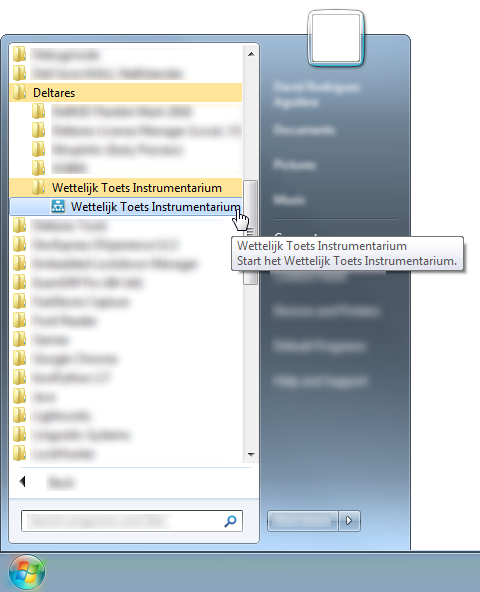
\includegraphics{figures/chapter_installation/rtInAllPrograms}
	\caption{Ringtoets in de startmenustructuur van Windows \color[rgb]{1,0,0} \textbf{Needs to be updated!!!}\color[rgb]{0,0,0}.}
	\label{fig:fig2.2}
\end{figure}


Kort nadat het programma ge\"instaleersd is, is deze snelkoppeling direct te vinden onder het startmenu:


\begin{figure} [H]
	\centering
		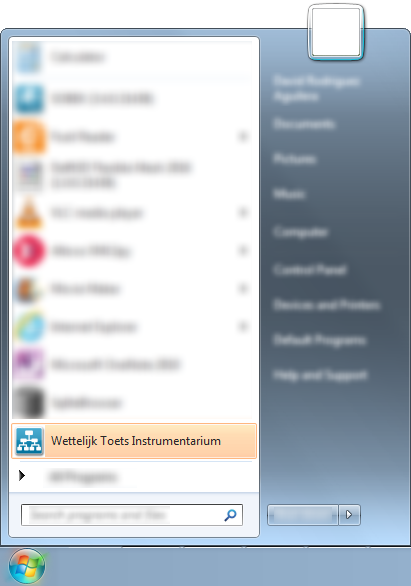
\includegraphics{figures/chapter_installation/rtDirectlyinStartMenu}
	\caption{Ringtoets direct in het startmenu van Windows \color[rgb]{1,0,0} \textbf{Needs to be updated!!!}\color[rgb]{0,0,0}.}
	\label{fig:fig2.3}
\end{figure}













